\documentclass[11pt, a4paper]{article}
\usepackage[utf8]{inputenc}
\usepackage[cjk]{kotex}
\usepackage{minted}
\usepackage{enumitem}
\usepackage{amsfonts}
\usepackage{amsmath}
\usepackage{graphicx}
\usepackage{fontspec}
\usepackage{hyperref}
\usepackage[a4paper, total={6in, 8in}]{geometry}

\title{HW 5: Ray Tracer}
\author{2015-10337 장필식}
\date{June 11, 2018}

\begin{document}

\maketitle

\section{To Run}

프로그래밍 언어는 Rust를 사용했다. 
\url{https://www.rust-lang.org/en-US/install.html}에서 나와있는 방법대로, 터미널에 \texttt{curl https://sh.rustup.rs -sSf | sh} 를 입력하면 간단하게 설치가 가능하다.

Rust와 cargo가 설치되었으면 프로젝트 폴더로 들어가 다음을 실행한다.

\begin{minted}{text}
cargo run --release -- 1 1920 1080 3 output.png
\end{minted}

여기서 Program Argument들은 다음과 같다.

\begin{itemize}
  \item SCENE(1): 씬의 종류 (1에서부터 5까지, 오브젝트들이 한꺼번에 모여있는 씬은 1번째이다.)
  \item WIDTH(1920): 이미지의 너비
  \item HEIGHT(1080): 이미지의 높이
  \item SAMPLE\_RATE(3): supersampling rate (추후에 설명). supersampling을 끄려면 1로 설정하면 된다.
  \item OUTPUT(output.png): 아웃풋 파일의 경로.
\end{itemize}

작업이 끝난 후에는 이미지가 프로젝트 폴더에 result.png로 나올 것이다.

\section{Dependencies}

프로그램에 사용한 패키지들은 다음과 같다. (Rust 패키지 목록은 프로젝트의 \texttt{Cargo.toml}에서 확인할 수 있다.)

\begin{itemize}
  \item cgmath: 선형대수 라이브러리.
  \item image: 이미지 입출력 관련 기능들.
  \item rayon: 멀티스레딩 라이브러리.
  \item tobj: obj 파일 로더 (간단한 텍스트 파싱만 지원한다.)
  \item clap: Argument parsing
  \item pbr: 진행 상태를 나타내주는 Progress Bar. (렌더링에서의 PBR이 아니다...)
  \item rand, chrono, itertools: 기타 자잘한 Rust 유틸리티등.
\end{itemize}

\section{Result}

기능 목록 중에 과제 스펙 이외에 추가로 구현한 가능들에은 별표를 붙였다.

\begin{figure}[H]
  \centering
  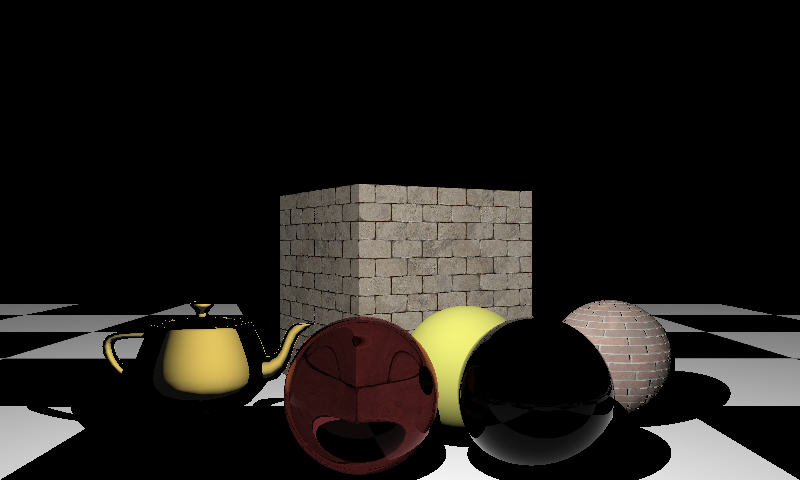
\includegraphics[width=0.9\textwidth]{final.png}
  \caption{final.png: 기능들을 모두 종합하여 만든 이미지.}
  \texttt{cargo run --release -- 1 1920 1080 3 final.png}
\end{figure}

위의 사진에서 각각의 물체가 나타내는 것들:

\begin{itemize}
  \item Ray tracing spheres \& polygons (주전자와 정육면체 모두 삼각형의 집합인 Mesh로 표현하여 렌더링했다.)

  \item Recursive reflection \& refraction
    \begin{itemize}
      \item 왼쪽에서 1번째 구는 reflection와 refraction을 동시에 하고 있다. (\texttt{reflection=1.0, refraction=0.5, color=rgb(0.9, 0.32, 0.36), refractive index=1.1})
      \item 왼쪽에서 3번째 구는 reflection만 하고 있다. (\texttt{reflection=1.0, refraction=0.0, color=rgb(0.9, 0.9, 0.9)}) 약간 어둡긴 하지만, 밑에 바닥 타일이 반사되고 있는 것을 관찰할 수 있다.
    \end{itemize}

  \item Phong illumination (Specular한 효과는 이 이미지에서 확인하기 어려울 수 있는데, 밑의 사진들에서 더욱 자세히 알아볼 것이다.)

  \item OBJ file loading (주전자): \texttt{resources/teapot.obj}를 로딩하였다.

  \item Image file exporting: \texttt{final.png} 생성됨.

  \item Texture mapped spheres and polygons:
    \begin{itemize}
      \item 정육면체: \texttt{resources/brickwall.jpg, reosurces/brickwall\_normal.jpg} 사용
      \item 주전자: \texttt{resources/Brick\_Wall\_012\_COLOR.jpg}, \texttt{resources/Brick\_Wall\_012\_NORM.jpg} 사용
      \item 바닥 타일: \texttt{resources/checker.png} 사용
    \end{itemize}

  \item Normal mapping (*): 벽돌 텍스쳐의 굴곡들을 더욱 실감나게 보여주기 위해 Normal mapping을 사용하였다. 고전적으로는 Bump mapping을 써서 이 문제를 해결했지만, 요즘에는 uv 좌표당 노말벡터가 이미지의 rgb값으로 담겨있는 normal map를 더욱 많이 볼 수 있다. (일단 더욱 예쁜 결과를 내주고, 인터넷에서 bump map보다 normal map을 찾기 훨씬 쉽기 때문에 사용했다.) 이것을 눈으로 한번에 구분하는게 힘들 수 있기 때문에, 밑의 사진들에서 더욱 자세히 알아볼 것이다.)

  \item Supersampling (*): 레이 트레이싱의 문제점 중 하나는 픽셀당 광선 하나를 쏘기 때문에, 물체들의 경게선들 부근의 픽셀들이 부드럽게 이어져 있지 않을 수 있다는 것이다. 이것을 해결하는 알고리즘은 다양하지만, 여기서 우리는 가장 간단하고 정확한 방법으로 기존 이미지보다 n배 더 크게 렌더링한 다음 n*n크기의 cell의 픽셀들의 색을 평균하여 다시 한 픽셀로 줄이는 방식으로 이미지를 더욱 부드럽게 만든다. (위 이미지에서 sample rate는 3이다.)
    
  \item Multithreaded (*): rayon 라이브러리를 사용해서 여러 개의 스레드에서 돌아갈 수 있게끔 하였다. (컴퓨터의 CPU 코어 수에 따라 자동으로 스레드 수가 설정한다.) 스레드의 개수에 따라 성능이 거의 비례한다는 것을 측정했다 (Intel(R) Core(TM) i7-6700HQ CPU @ 2.60GHz 에서 측정).
    \begin{itemize}
      \item 1개의 스레드 (\texttt{cargo run --release -- --single-thread 1 1920 1080 1 output.png}): 121.281s
      \item 8개의 스레드 (\texttt{cargo run --release -- 1 1920 1080 1 output.png}): 17.063s (7.1배 빠름)
    \end{itemize}

\end{itemize}


\begin{figure}[H]
  \centering
  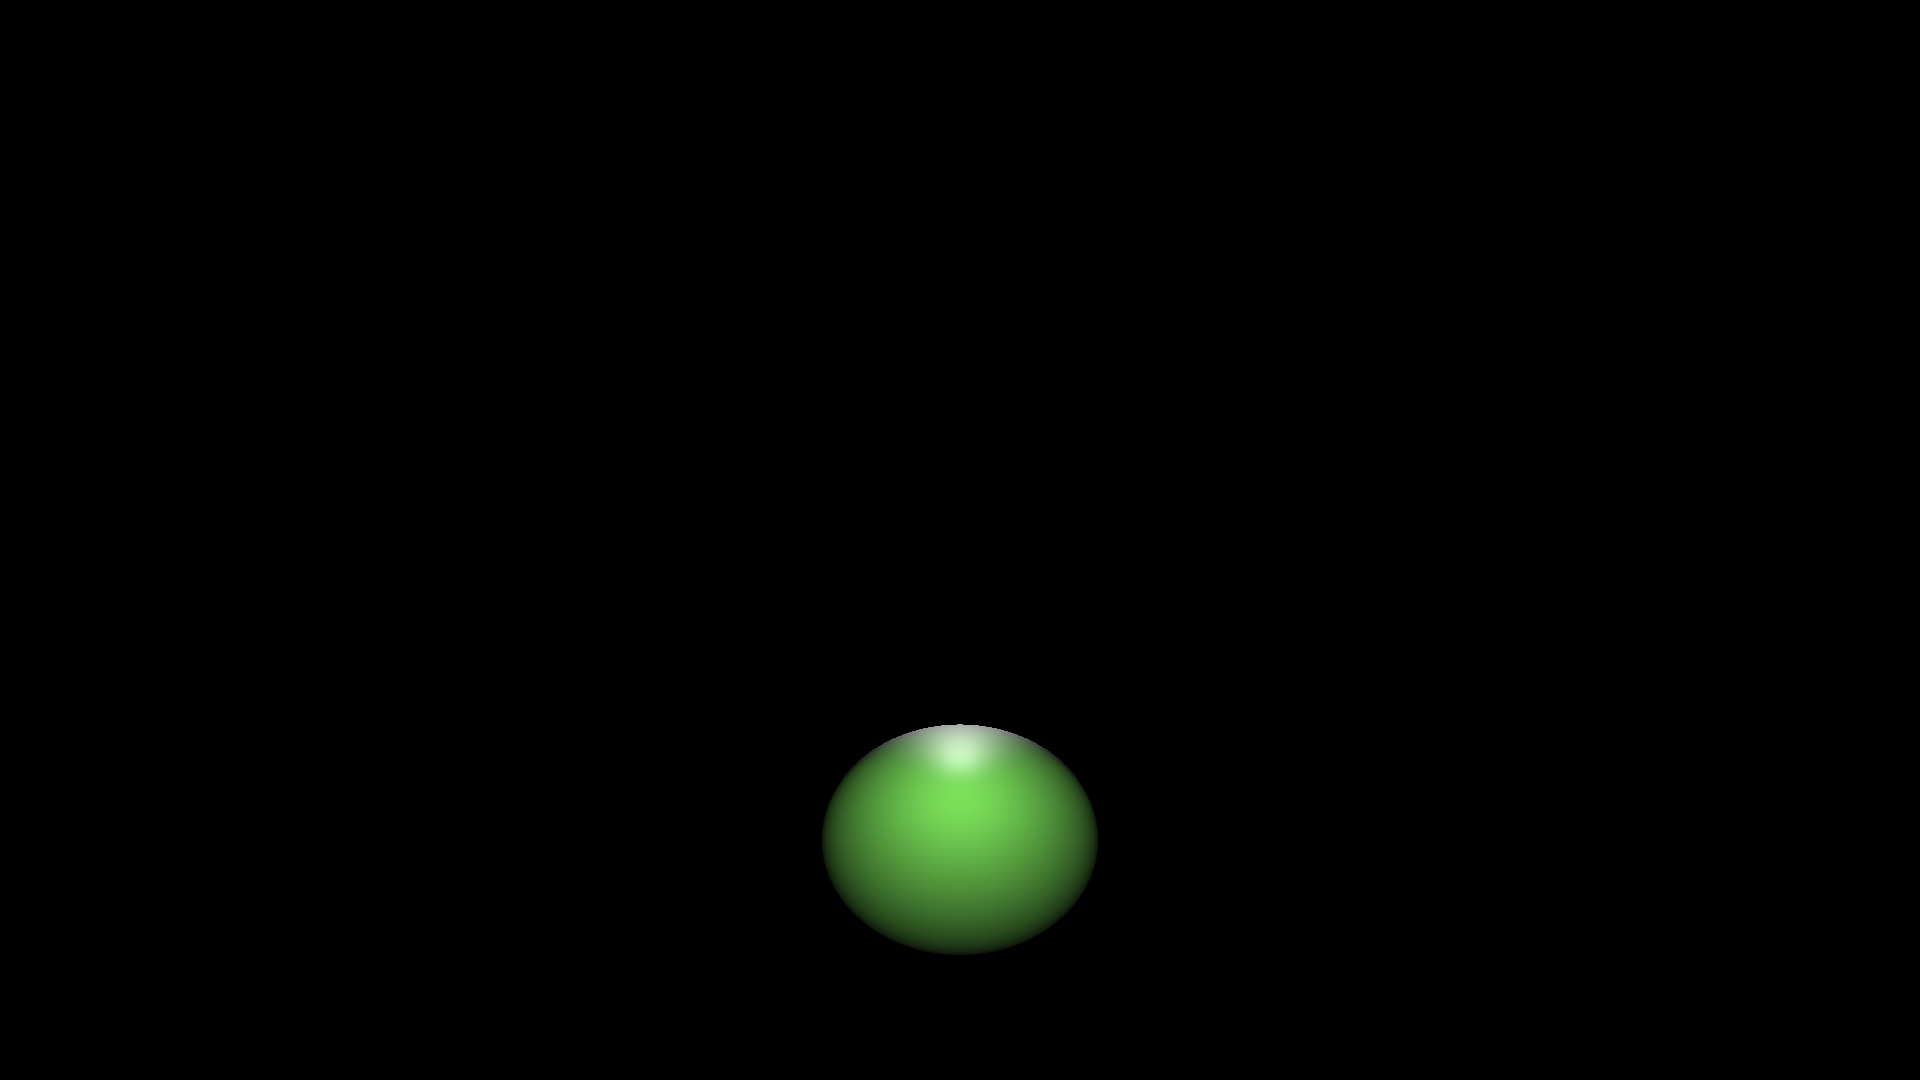
\includegraphics[width=0.9\textwidth]{specular.png}
  \caption{specular.png: Specular lighting 효과 재현.}
  \texttt{cargo run --release -- 5 1920 1080 1 specular.png}
\end{figure}

Specular lighting의 효과를 위 렌더링 결과에서 볼 수 있다.

\begin{figure}[H]
  \centering
  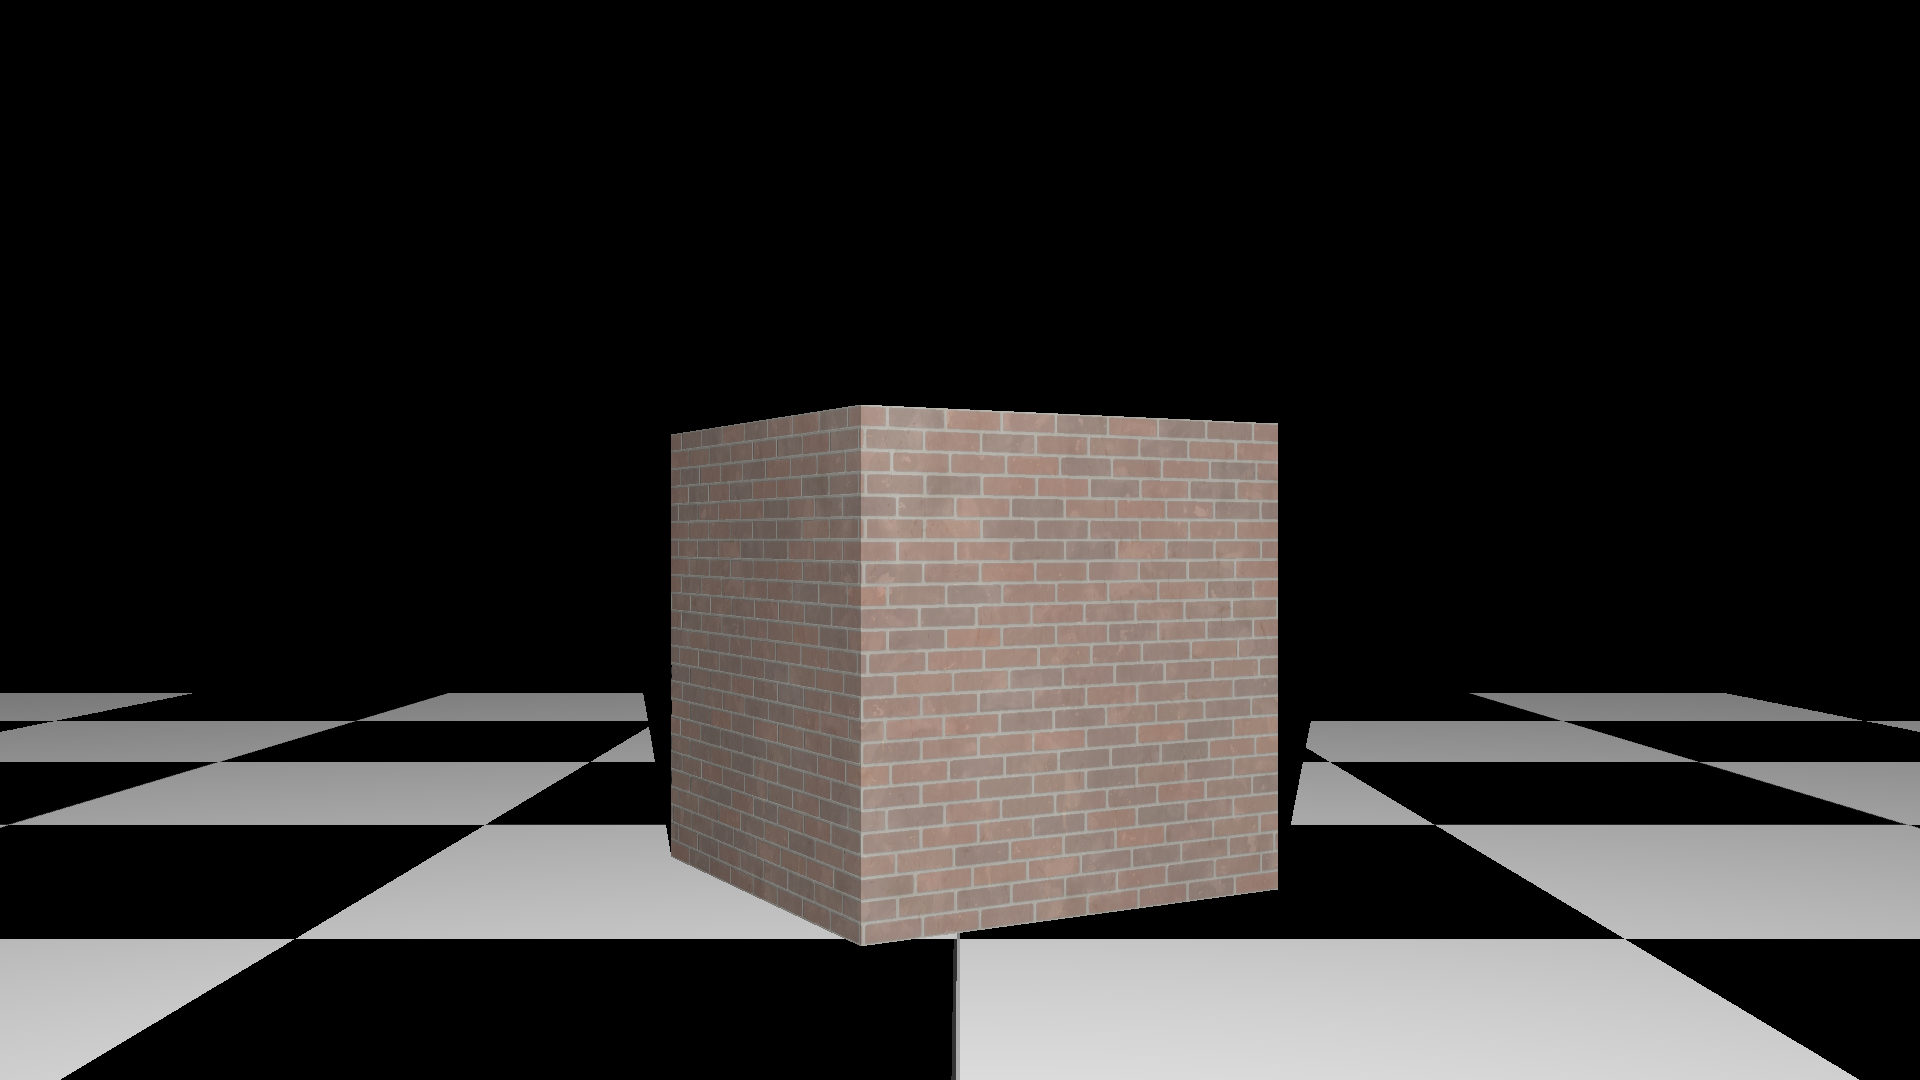
\includegraphics[width=0.9\textwidth]{cube-with-normal.png}
  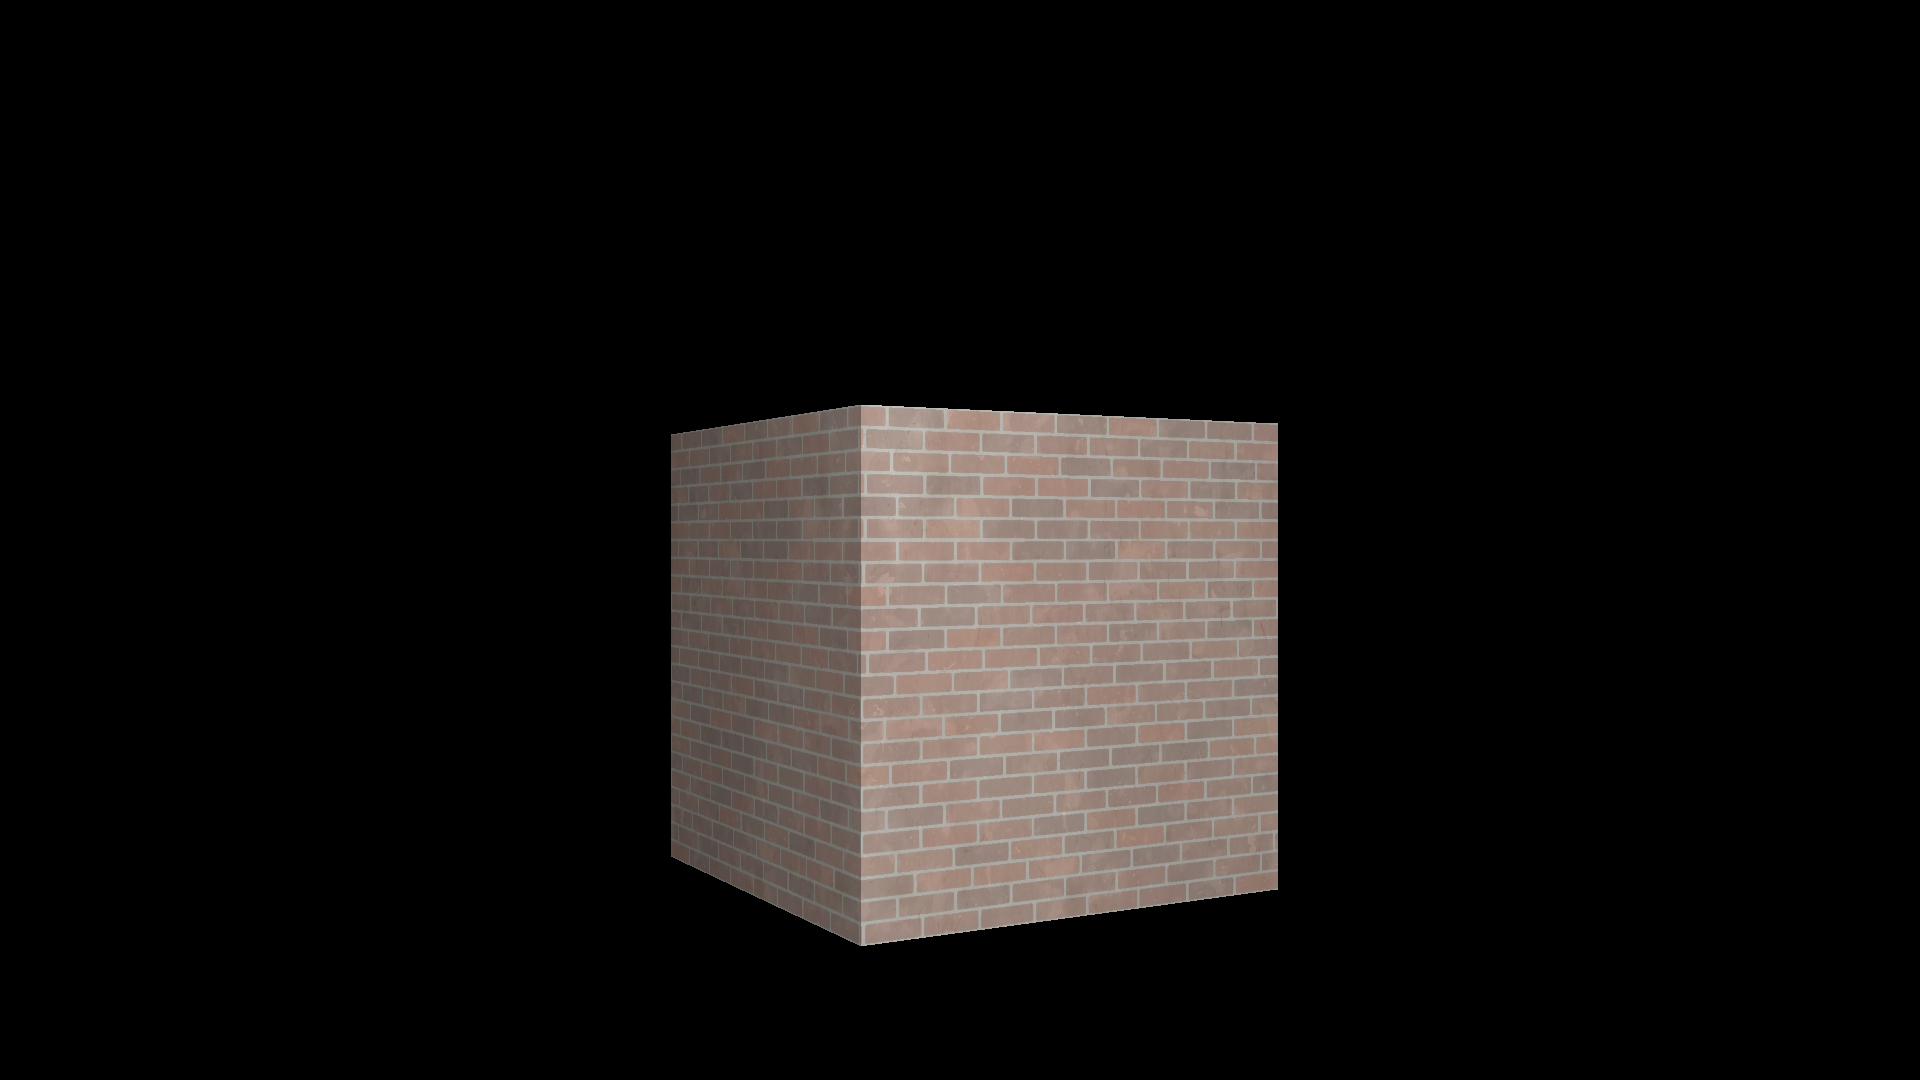
\includegraphics[width=0.9\textwidth]{cube-without-normal.png}
  \caption{cube-with-normal.png vs cube-without-normal.png: Normal mapping을 적용한 이미지와 그렇지 않은 이미지의 비교.}

  \texttt{cargo run --release -- 3 1920 1080 1 cube-with-normal.png}

  \texttt{cargo run --release -- 4 1920 1080 1 cube-without-normal.png}
\end{figure}


Normal mapping이 되어있는지를 더욱 자세히 확인하기 위해서 다음과 같이 두 사진을 비교해 보았다. 자세히 보면 윗쪽의 그림이 아래쪽 그림보다 벽돌들 사이의 굴곡들이 더 자세히 표현되었다는 것을 알 수 있다.

\begin{figure}[H]
  \centering
  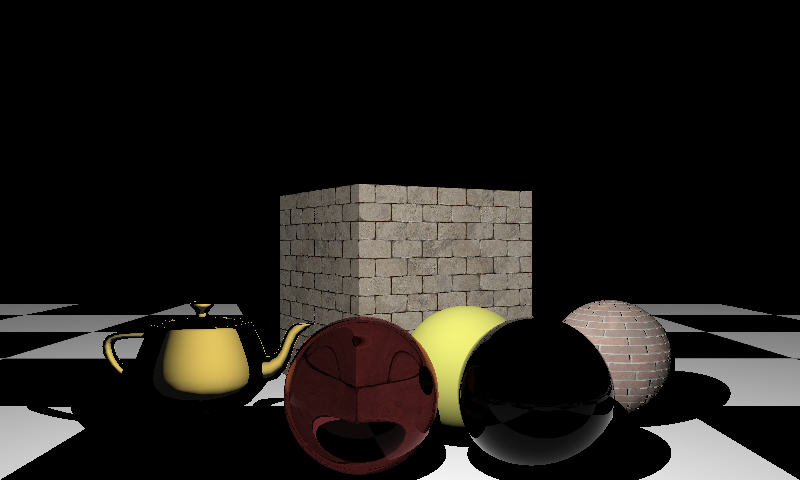
\includegraphics[width=0.9\textwidth]{final.png}
  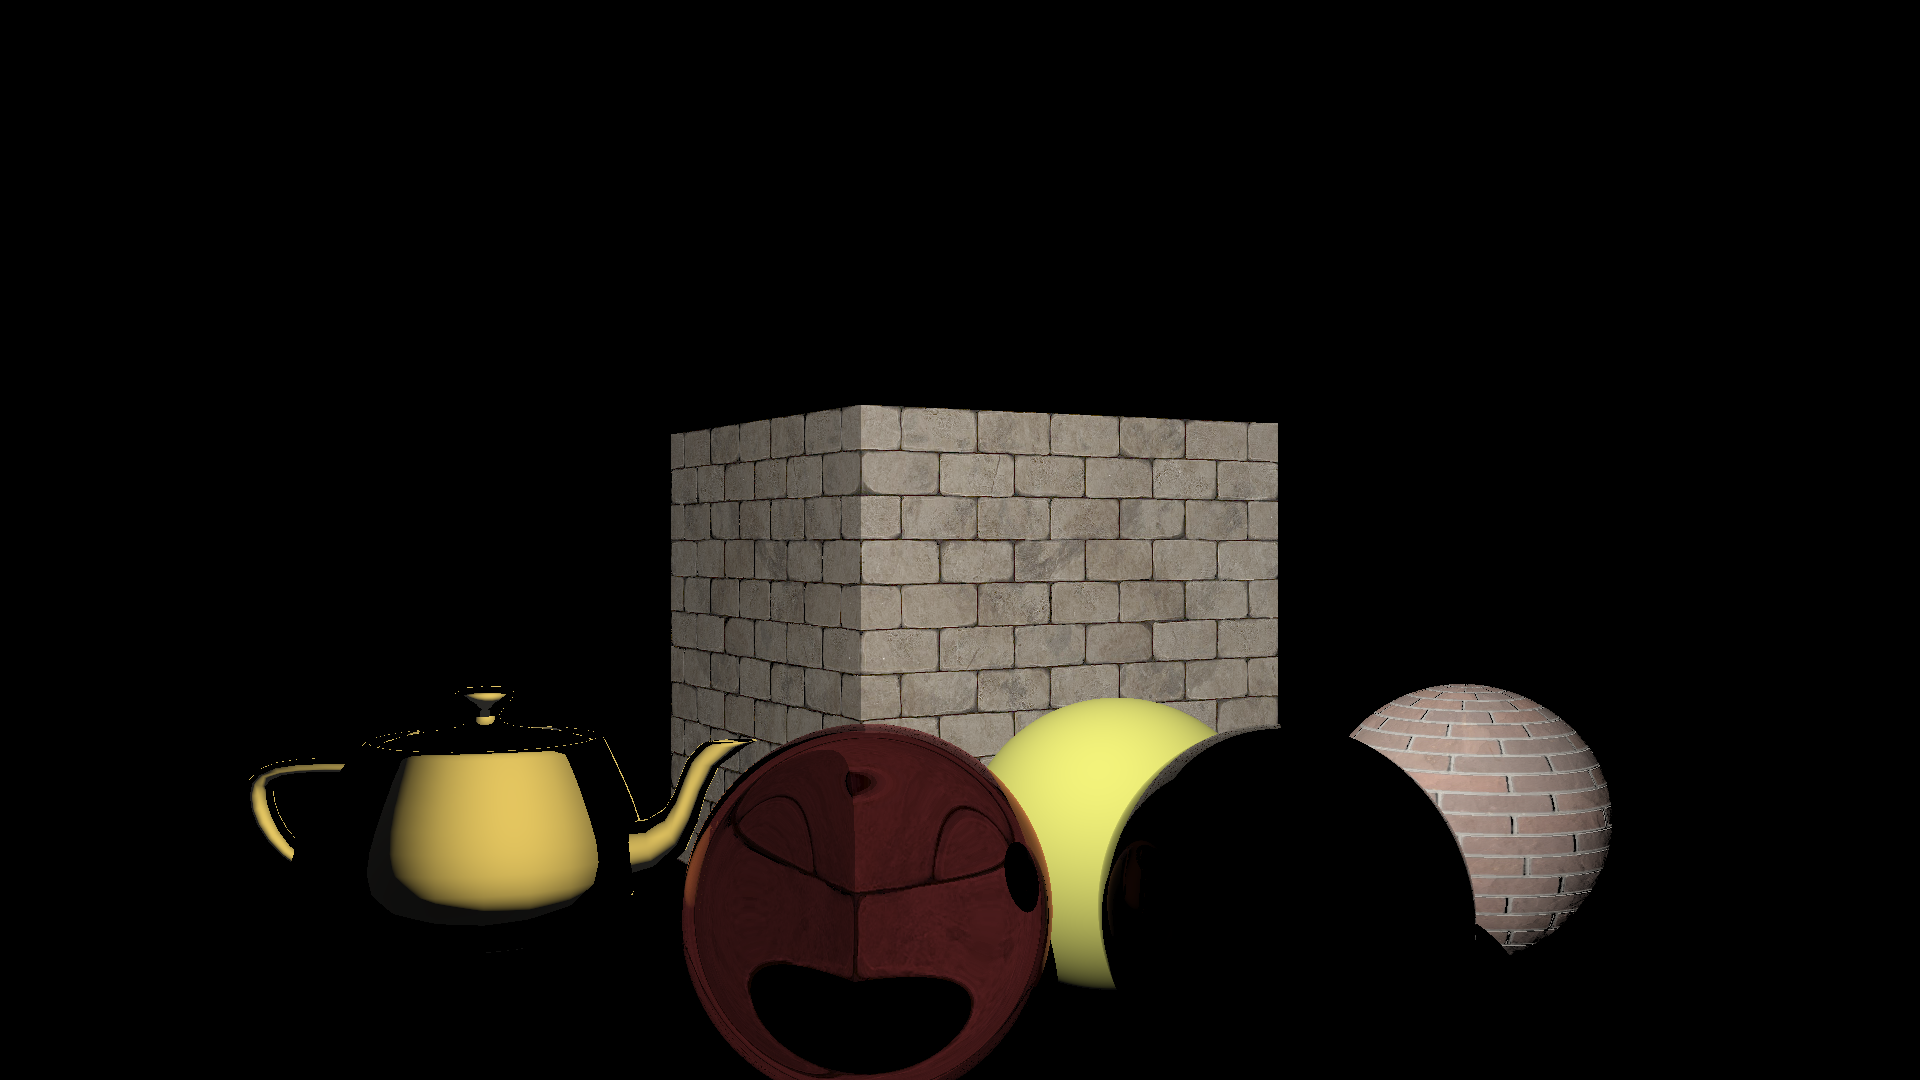
\includegraphics[width=0.9\textwidth]{final-no-supersampling.png}
  \caption{final.png vs final-no-supersampling.png: Supersampling을 적용한 이미지와 그렇지 않은 이미지의 비교.}
  \texttt{cargo run --release -- 1 1920 1080 3 final.png}

  \texttt{cargo run --release -- 1 1920 1080 1 final-no-supersampling.png}
\end{figure}

비슷한 방법대로 Supersampling을 적용한 사진과 적용하지 않은 두 사진을 비교해 보았다. 위쪽의 그림의 경계선들이 더 매끄럽다는 것을 알 수 있다.

이외의 사진들 (\texttt{spheres1.png} 부터 \texttt{spheres6.png} 까지) 는 ray tracer를 제작하는 과정 속에서 만든 이미지들을 순서대로 나열해 놓은 것이다. 여기서는 좀 더 다양한 refraction 효과를 주로 관찰할 수 있다.

\end{document}
